\documentclass[preprint]{JHEP3} % 10pt is ignored!

\JHEPspecialurl{http://jhep.sissa.it/JOURNAL/JHEP3.tar.gz}
\usepackage{graphicx}
\usepackage{amsmath,amssymb}
\usepackage{cite}
\usepackage{multirow}

%\newcommand{\DF1A}{\Delta F_{1,A}}
%\newcommand{\DF1V}{\Delta F_{1,V}}
%\newcommand{\Dphill}{\Delta \phi_{ll}}
\newcommand{\eps}{\epsilon}
\newcommand{\mrm}{\mathrm}
\def\DF1A{\Delta F_{1,A}}
\def\DF1V{\Delta F_{1,V}}
\def\Dphill{\Delta \phi_{ll}}
\def\ttbZ{t\bar{t}Z}
\def\ttb{t\bar{t}}
\def\ptZ{p_{t,Z}}
\newcommand{\be}{\begin{eqnarray}}
\newcommand{\ee}{\end{eqnarray}}
%\newcommand{\ttb}{t \bar{t}}

\title{Constraining top-Z coupling through $t\bar{t}Z$ production at the LHC}

\author{Raoul R\"ontsch \\ Fermilab, Batavia, IL 60510, USA \\
  Email: \email{rontsch@fnal.gov} }
\author{Markus Schulze}


\received{\today} 		%%
%\revised{}
\accepted{\today}		%% These are for published papers.


\preprint{}

\abstract{We constrain top-Z coupling through ttbZ at LHC.}

\begin{document}
%\maketitle
\section{Introduction}
After a highly successful lower energy run at $\sqrt{s}=7$ and $8$ TeV, the Large Hadron Collider (LHC) is now on shutdown in preparation for a longer run at a higher energy of $\sqrt{s}=13$ or $14$ TeV. This affords the high energy physics community the opportunity to examine the possible future physics reach of the LHC. The large top quark production rate at the LHC has allowed detailed study of several of it properties. A combined ATLAS and CMS analysis \cite{ATLAS-CONF-2013-102} has measured the top mass with an accuracy comparable to that obtained at the Tevatron \cite{}. The top electric charge \cite{Aad:2013uza}, $\ttb$ charge asymmetry \cite{CMS-PAS-TOP-12-033}, and $\ttb$ mass difference \cite{Aad:2013eva} have also been measured recently. {\bf top quarks w dijet?}. 

The large top mass places it in a special position within the electroweak symmetry breaking framework. For this reaon, a direct determination of the coupling of the top quarks to the massive gauge bosons would be extremely interesting.  A significant deviation from the Standard Model (SM) value could be indicative of new physics {\bf some silly susy example here? I don't think its a good idea...}; on the other hand, confirmation of the SM value would place further constraints on any new physics scenario. Both CMS \cite{Chatrchyan:2013qca} and the ATLAS \cite{ATLAS-CONF-2012-126} have observed top-pair events produced in association with a vector boson, albeit with very low statistics. The question then arises: how well can the upcoming run at higher energy and larger luminosity constrain the top-vector boson coupling?

In this paper, we will focus on the ability of the LHC to determine the top-$Z$ coupling through $\ttbZ$ production. The $\ttbZ$ coupling is already measured by indirect means, through the decay of {\bf ??? and ref}, which heavily disfavors a non-SM value. It is worthwhile to attempt to corroborate this measurement using direct means. {\bf flesh this out -- some numbers???}

The ability of the LHC to constrain the top-$Z$ coupling was first considered in ref. \cite{Baur:2004uw,Baur:2005wi}. The transverse momentum of the $Z$ boson $\ptZ$ and the azimuthal angle between the leptons originating from its decay $\Dphill$ were found to be sensitive to this coupling. This observation, together with the desirability of applying realistic experimental cuts, means that our analysis must take into account the decays of the top quarks and the $Z$ bosons, including all spin correlations. Furthermore, the authors of ref. \cite{Baur:2004uw,Baur:2005wi} identified the large leading order (LO) scale uncertainty in the theoretical predictions as the main obstacle to tighter constraints on the top-$Z$ coupling. To reduce this uncertainty, we perform our calculation to next-to-leading order (NLO) in QCD, including the NLO corrections to the top quark decay products. {\bf something about the paper of Berger et al}

The production of $\ttbZ$, with stable tops and $Z$ boson, has been previously was studied at NLO accuracy by Lazopoulos, McElmurry, Melnikov, and Petriello \cite{Lazopoulos:2008de}, and  by Kardos, Papadopoulos, and Trocsanyi \cite{Kardos:2011na}. Disagreement at the level of 3\% of the cross-section, and a small shape difference in $\ptZ$, was found between these two calculations. The latter calculation was also interfaced to a parton shower \cite{Garzelli:2011is}, performing the decays of the top quarks and $Z$ boson through the parton shower. This neglects the contribution from the NLO corrections to the top decays, which are included in our calculation. Furthermore, the parton showering produces isotropic distributions and cannot be used to compare spin-dependent observables, such as the lepton opening angle.  This paper then presents the first calculation of NLO effects in $\ttbZ$ production and decay, and including all spin correlations.

The study of top-Z coupling is not the only scenario in which the $\ttbZ$ process is interesting. The invisible decay $Z \to \nu \bar{\nu}$ produces a signature of a top pair plus a large amount of missing transverse energy, and is therefore an irreducible background to stop searches. While we do not address this issue in this paper, it would be interesting to study the effects of the NLO corrections on this background, using cuts typical of a stop search. {\bf some refs? how is this taken into accoutn? surely not data extrapolation, so must be MC, in which case NLO corr important?}

The top-$Z$ coupling may also be directly probed through single top production in association with a $Z$-boson. While the inclusive cross-section of $tZ$ plus its charge conjugate process $\bar{t}Z$ is comparable to the inclusive $\ttbZ$ cross-section \cite{Campbell:2013yla}, it should be possible to separate these processes by cutting on forward jets and demanding a high jet multiplicity. We will therefore consider only the $\ttbZ$ process in this paper, and defer the study of the coupling using $tZ+\bar{t}Z$ (or both this and $\ttbZ$) to a later date.

% Pheno motivation: LHC a top factory, new top measurements; possibility of measuring top couplings; ttbZ $\to \nu \nu$ as background to MET searches for stops. \\
% Previous NLO calc (w/o top or Z decay): LMMP, KTP \\
% Prev. analysis of top-Z couplings: Baur et al, Berger et al \\
% Comparison with indirect constraints on top-Z coupl \\
% Single top+Z \\

\section{Outline of calculation}
\subsection{NLO calculations}
In this section, we discuss some of the general features of the partonic calculation of $\ttbZ$ production and decay. We use the narrow-width approximation (NWA), allowing us to separate the production and decays of the top quarks. Since the phase space available for the decay $t \to WbZ$ is small, we consider radiation of the $Z$ boson to occur in the production amplitudes only. Our calculation then neatly factorizes into the production of $\ttbZ$ to NLO in QCD, and the decay of the tops and $Z$ to NLO in QCD.

At LO in QCD, the production of $\ttbZ$ occurs through the $gg$ and $q\bar{q}$ partonic channels. At NLO, these channels receive real and virtual corrections, while real emission corrections also open the partonic channels $qg$ and $\bar{q}$. The virtual corrections are calculated using an OPP realization \cite{Ossola:2006} of  $D$-dimension generalized unitarity \cite{Ellis:2007br,Giele:2008ve,Ellis:2008ir} (for a review, see \cite{Ellis:2011}). Included in the virtual corrections are fermion loops with top quarks circulating in the loop. The real emission corrections introduce infrared divergences due to the appearance of soft and/or collinear partons. We employ Catani-Seymour dipoles \cite{Catani:1996vz,Catani:2002hc} to remove these infrared divergences. 

The NLO amplitudes for the decay of the top quarks well-known, and are given in \cite{Jezabek:1988iv,Czarnecki:1990pe,Czarnecki:1990kv,Li:1990qf,Campbell:2004ch,}. In the NWA, the NLO cross-section for the production and decay is written as \cite{Campbell:2004ch,Melnikov:2009dn}
\begin{equation}
\begin{split}
d \sigma_{\ttbZ}^{\mrm{NLO}} =& (\Gamma_{\ttb,\mrm{tot}}^{LO})^{-2} \biggl[ d \sigma_{\ttbZ}^{\mrm{LO}} d\Gamma_{\ttb}^{\mrm{LO}} +  + d\Gamma_{\ttb}^{\mrm{LO}} \bigl( d\sigma_{\ttbZ}^{\mrm{virt}} +d\sigma_{\ttbZ+j}^{\mrm{real}} \bigr) \\ 
& + d \sigma_{\ttbZ}^{\mrm{LO}} \biggl(d\Gamma_{\ttb}^{\mrm{virt}}+d\Gamma_{\ttb+j}^{\mrm{real}}  - 2d\Gamma_{\ttb}^{\mrm{LO}} \frac{\Gamma_{\ttb,\mrm{tot}}^{\mrm{NLO}}}{ \Gamma_{\ttb,\mrm{tot}}^{\mrm{LO}}} \biggr) \biggr],
\end{split}
\end{equation}
{\bf Markus: do we use the last -2... term? I don't see it in eq. 3 of your ttbj paper, 1111.4991}
where $d\Gamma_{\ttb}$ includes the decay of the top and antitop quarks, and $\Gamma_{\ttb,\mrm{tot}}$ is the full top-pair decay width. The use of the NWA introduces errors $\mathcal{O}(\Gamma_t / m_t) \simeq 1\%$ \cite{AlcarazMaestre:2012vp}. These effects can affect large shape changes in distributions that are sensitive to the top mass, such as the mass of the bottom-$W$ system \cite{AlcarazMaestre:2012vp,Papanastasiou:2013dta}. Since we shall only concern ourselves with leptonic distributions and overall cross-sections, such effects do not warrant concern. We also employ the NWA in the leptonic decay of the $Z$ boson. We therefore neglect final state leptons which arise through an intermediate photon. Such effects are negligible if the a mass cut is placed on the lepton pair {\bf I think? I don't know of any refs... Also, this should introduce errors ~ 3 percent.}

We perform several checks on our calculations. The amplitudes for the Born and real emission corrections are checked against MadGraph \cite{Alwall:2011uj}. The singular structure of the virtual amplitudes is well-known analytically from the Catani-Seymour integrated dipoles, and our numerical value is checked against these. We also check the finite part of the virtual amplitude against the automated program {\tt GoSam} \cite{Cullen:2011ac}. In the dipole implementation of ref. \cite{Nagy:2003tz,Nagy:2003tz}, the singular phase space is controlled by a parameter $\alpha$. We have checked that our results, both for production and decay, are independent of this parameter. The factorization into a production and decay amplitude is checked by observing that the inclusive cross-section with top and $Z$ decays equal to the inclusive cross-section for stable tops and $Z$, multiplied by the branching ratios. {\bf any more?}

As mentioned previously, the $\ttbZ$ production has been calculated to NLO, for the case of stable tops and $Z$ boson. This calculation was first performed in ref.~\cite{Lazopoulos:2008de}. For completeness, we repeat the parameters used in that calculation. The masses of the top quark, $W$ boson and $Z$ are $m_t=170.9$ GeV, $m_W=80.45$ GeV, and $m_Z=91.19$ GeV. The electroweak coupling is defined through the Fermi constant $G_F$ and the weak mixing angle $\sin^2\theta_w = 1-m_W^2/m_Z^2 =0.2215$. The MSTW2004 parton distribution functions are used \cite{}, giving a strong coupling $\alpha_s(m_Z)=$ at LO and $\alpha_s(m_Z)=$ at NLO {\bf fill these in}. At the central factorization and renormalization scale of $\mu_0=m_t+m_Z/2$, the cross-section was found to be 808 fb at LO and 1090 fb at NLO, leading to a $k$-factor of 1.35. The calculation was repeated in ref.~\cite{Kardos:2011na}.  Using the same set of parameters as ref.~\cite{Lazopoulos:2008de}, agreement with the LO cross-section was found. However, the NLO cross-section was found to be 3\% higher at 1121 fb, giving a slightly larger $k$-factor of 1.39. 






%OPP, C-S dipoles, top decay at NLO, NWA for tops and Z + Refs \\
Leptonic, inclusive variables so no need for parton showering \\
%Checks: poles, factorization, alpha-param \\
Comparison with KTP, LMMP - cross-secs, distr \\

\subsection{Top-Z coupling}
Definition of top-Z couplings - vector, axial-vector, left and right handed \\
Focus of D=4 operators -- D=6 for later (unclear how to implement unitarity for such operators) \\
Definition of DF1V and DF1A

\section{Results}
\subsection{NLO Results}
Four distr incl scale bounds (incl at least one of a decay product) at LO, NLO\\
Comparison with NLO + LO decay \\
Comparison with 0+1 jet from MadGraph using CKKW merging \\
Acceptance function = $\sigma_{\mathrm{incl}} / \sigma_{\mathrm{cuts}}$ at LO, NLO\\
Point out large k-factor with cuts than with fully inclusive \\

LO and NLO cross sections for acceptance cuts given in eq.~\ref{}
\be
  \sigma_{\ttb Z}^\mathrm{LO} &= 3.80^{+1.31}_{-0.94}~\mathrm{fb},
  \quad\quad\quad
  \sigma_{\ttb Z}^\mathrm{NLO} &= 5.32^{+0.78}_{-0.74}~\mathrm{fb}
\\
% 
  \sigma_{\ttb Z}^\mathrm{LO} &= 3.80^{+34\%}_{-25\%}~\mathrm{fb},
  \quad\quad\quad
  \sigma_{\ttb Z}^\mathrm{NLO} &= 5.32^{+15\%}_{-14\%}~\mathrm{fb}
\\
% 
  \sigma_{\ttb Z}^\mathrm{LO} &= 3.98 \pm 28\% ~\mathrm{fb},
  \quad\quad\quad
  \sigma_{\ttb Z}^\mathrm{NLO} &= 5.34 \pm 14 \%~\mathrm{fb}
\ee
Results are represented in three ways (need to pick one).
We also calculate the cross section without acceptance cuts and find
\be
  A^\mathrm{LO} = \frac{\sigma_{\mathrm{cuts}}^\mathrm{LO}}{\sigma_{\mathrm{total}}^\mathrm{LO}} = 27.2 \% ,
  \quad\quad\quad
  A^\mathrm{NLO} = \frac{\sigma_{\mathrm{cuts}}^\mathrm{NLO}}{\sigma_{\mathrm{total}}^\mathrm{NLO}} = 30.5 \%.
\ee

\subsection{Top-Z coupling results}
Constraints from $t\bar{t}Z$ cross-section from CMS \\
Dphill distr with LO and NLO scale bands, and two(three?) non-SM coupl\\
$\sigma_{NP|} / \sigma_{SM}$ a la Berger, 0907.2191 \\
Description of analysis Binned log likelihood, how we handle scale uncertainty (cf. Lykken et al) \\
alpha plots - LO, NLO, rescaled (k-factor and reduced scale uncertainty) LO at 30, 300, 3000 fb-1\\
Dphill distr normalized to $t\bar{t}$ cross-section  - 1 uncertainty from k-factors at 30, 300, 3000\\

\section{Conclusion}
Future work: extension to dim 6 operators, incl single top + Z results, more advanced analysis techniques (e.g. MEM), e+e- collider.
%


\acknowledgments
We acknowledge helpful conversations with A.~Gritsan, N.~Tran and P.~Argrawal. 



\appendix
\section{plots}
Temporariy repository for plots.


\begin{figure}[h]
\centering % \begin{center}/\end{center} takes some additional vertical space
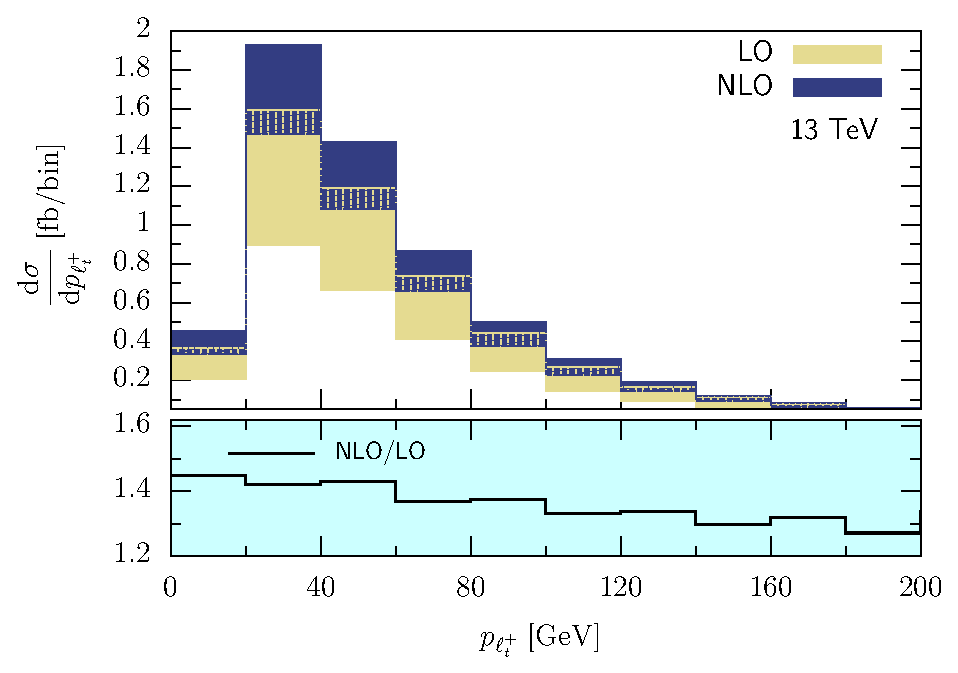
\includegraphics[width=0.45\textwidth]{./LHC_53_Fig01.eps}
\hfill
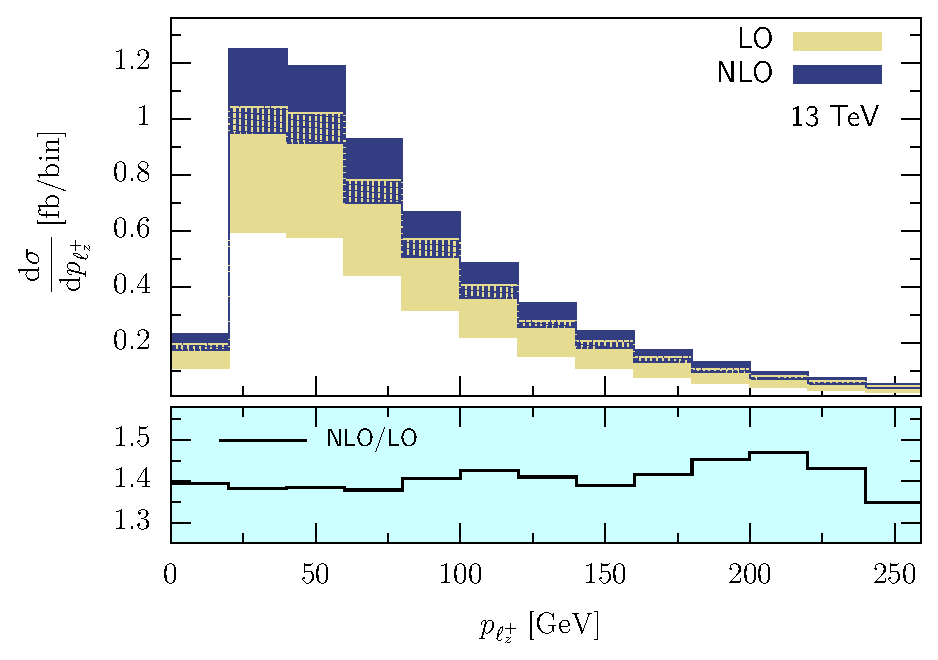
\includegraphics[width=0.45\textwidth]{./LHC_53_Fig03.eps}
\caption{\label{fig:i} Caption here.}
\end{figure}


\begin{figure}[h]
\centering % \begin{center}/\end{center} takes some additional vertical space
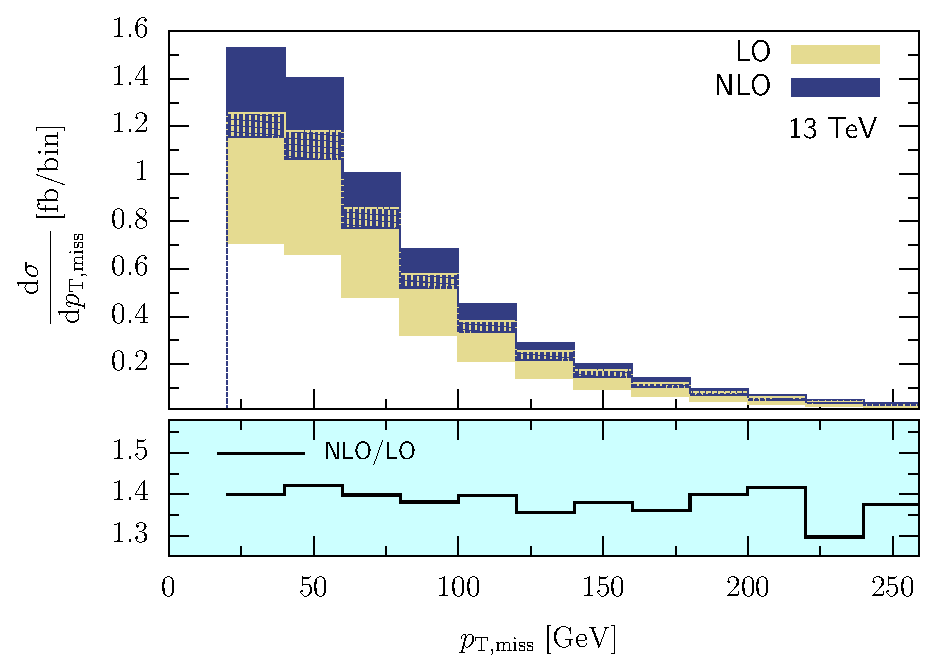
\includegraphics[width=0.45\textwidth]{./LHC_53_Fig08.eps}
\hfill
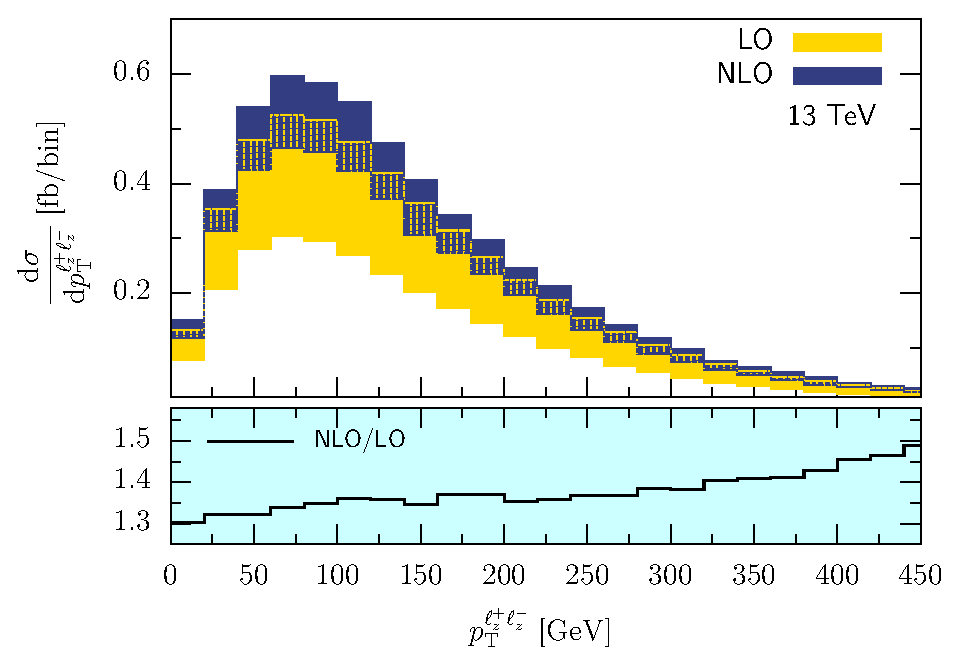
\includegraphics[width=0.45\textwidth]{./LHC_53_Fig12.eps}
\caption{\label{fig:i} Caption here.}
\end{figure}



\begin{figure}[h]
\centering % \begin{center}/\end{center} takes some additional vertical space
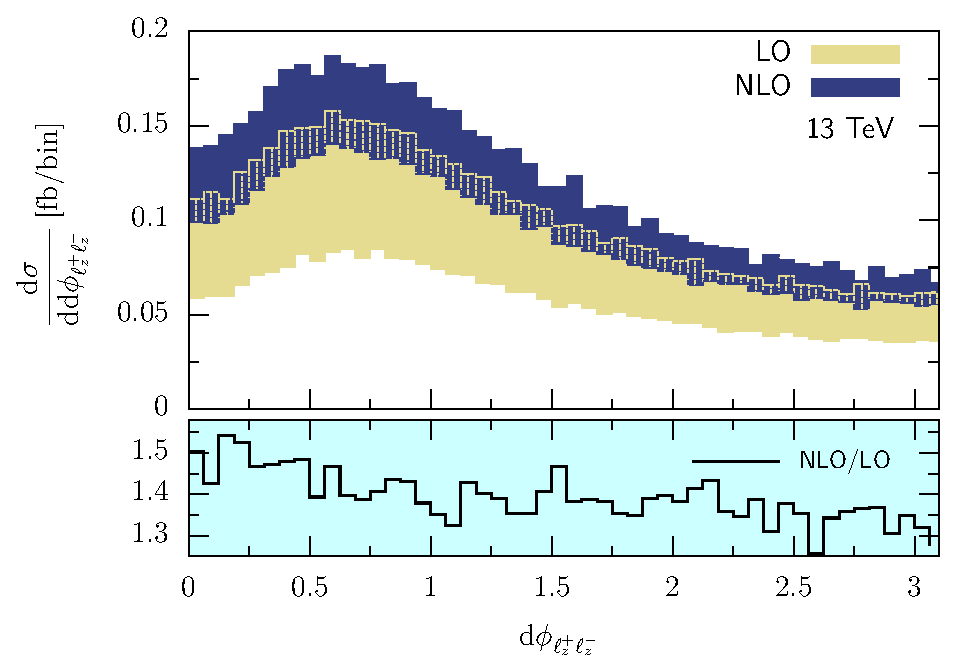
\includegraphics[width=0.45\textwidth]{./LHC_53_Fig17.eps}
\hfill
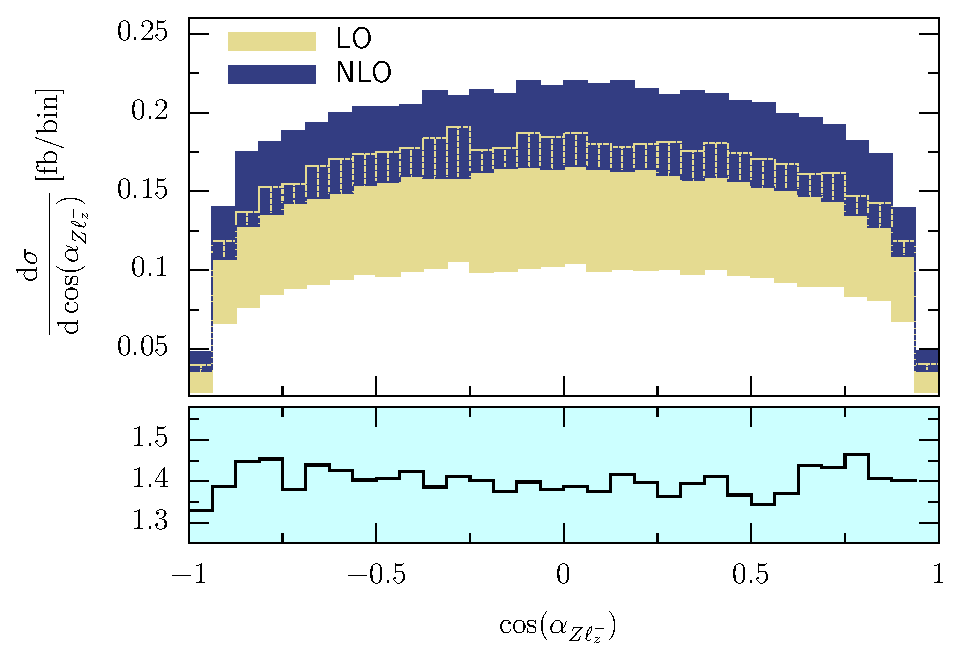
\includegraphics[width=0.45\textwidth]{./LHC_53_Fig18.eps}
\caption{\label{fig:i} Caption here.}
\end{figure}




\begin{figure}[h]
\centering % \begin{center}/\end{center} takes some additional vertical space
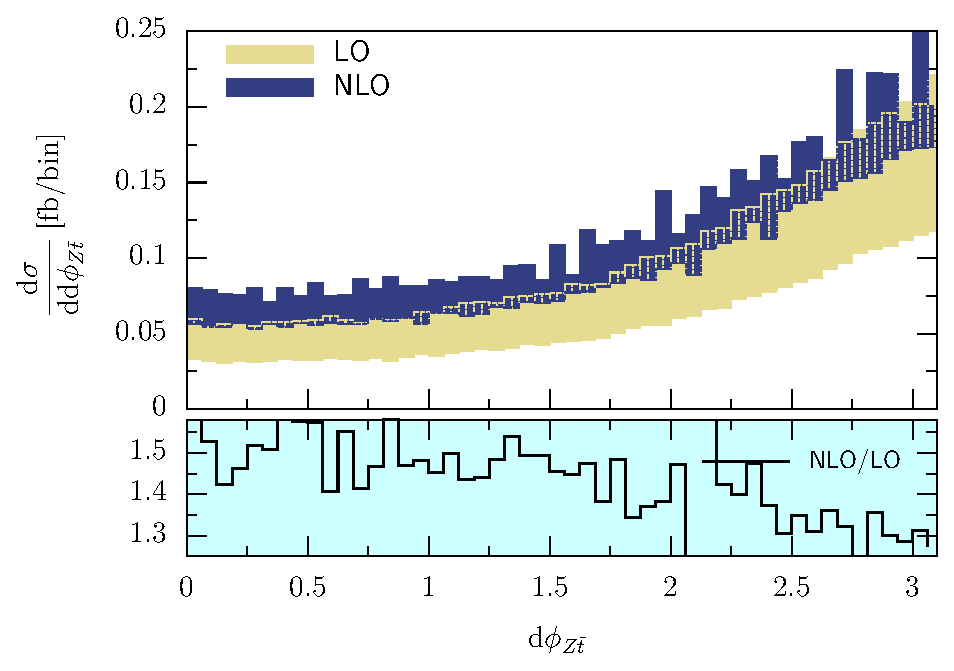
\includegraphics[width=0.45\textwidth]{./LHC_53_Fig19.eps}
\caption{\label{fig:i} Caption here.}
\end{figure}


\bibliographystyle{JHEP}
\bibliography{ttbZ}

%\begin{thebibliography}{99}

%\cite{Campbell:2013yla}
%\bibitem{Campbell:2013yla} 
%  J.~Campbell, R.~K.~Ellis and R.~Rontsch,
%  %``Single top production in association with a Z boson at the LHC,''
%  Phys.\ Rev.\ D {\bf 87}, 114006 (2013)
%  [arXiv:1302.3856 [hep-ph]].
%  %%CITATION = ARXIV:1302.3856;%%
%\end{thebibliography}

\end{document}








